\documentclass[10pt]{article}
% Workshop draft. Swap the preamble for the venue's style file (e.g. ICBINB / ICLR) before submission;
% the body uses only standard packages.
\usepackage[margin=1in]{geometry}
\usepackage[utf8]{inputenc}
\usepackage[T1]{fontenc}
\usepackage{amsmath,amssymb}
\usepackage{booktabs}
\usepackage{graphicx}
\usepackage{xcolor}
\usepackage[numbers,sort&compress]{natbib}
\usepackage[colorlinks=true,linkcolor=blue!50!black,citecolor=blue!50!black,urlcolor=blue!50!black]{hyperref}

\graphicspath{{../results/figures/}}
\newcommand{\E}{\textsc{E}}

\title{Structure Is Not Enough: A Pre-registered Test of\\Hamiltonian World Models for Control}
\author{Shushant Kumar Choudhary\\\texttt{shushant1771@gmail.com}}
\date{}

\begin{document}
\maketitle

\begin{abstract}
Hamiltonian neural networks conserve energy by construction, which suggests that a world model whose
latent dynamics are Hamiltonian should predict further, generalise to unseen energies, and support more
sample-efficient control than models that learn physics through a loss or not at all. We tested this
claim with four hypotheses, thresholds and decision rules that were frozen in a pre-registration before
any model code existed. We compared an action-conditioned, port-Hamiltonian world model (symplectic
latent step, learned control input and damping) against an MLP, a privileged PINN, an energy-penalised
latent Neural ODE and an RSSM on four simulated systems with exactly known energy (60 state-vector runs,
18 pixel model-based RL runs). None of the four hypotheses is supported. The model conserves its
\emph{own} learned energy to $10^{-5}$--$10^{-2}$ over 10,000 steps, but whenever the learned Hamiltonian
is wrong away from the data the latent trajectory slides, at constant learned energy, into states with
the wrong true energy (drift 37 to 14,000 on 5 of 9 runs; the latent ODE stays at 0.15--1.2 except on the two seeds where
its rollouts diverge). Its
2$n$-dimensional canonical bottleneck also costs one to three orders of magnitude in one-step error,
and on the chaotic acrobot it never beats the best baseline at any horizon. We report the null results,
the two pre-registered amendments and what they cost, and an independent replication of the result
that an energy penalty helps a latent ODE on the two-body problem.
\end{abstract}

\section{The belief}

A recurring argument for physics-structured models is that structure beats a loss: a network whose
dynamics are Hamiltonian by construction \citep{greydanus2019hnn,toth2020hgn,zhong2020symoden} cannot
violate energy conservation, whereas a network with an energy penalty \citep{raissi2019pinn} only
approximately obeys it. Applied to world models
\citep{ha2018worldmodels,hafner2019planet}, the argument predicts that a Hamiltonian latent space should
give (i) bounded long-horizon energy error, (ii) better extrapolation to energies outside the training
band, (iii) more sample-efficient model-predictive control, and (iv) on a chaotic system, an advantage
that holds for about one Lyapunov time and then disappears, because no model can beat chaos.

We wrote these down as four quantitative hypotheses (H1--H4, Table~\ref{tab:verdicts}) with thresholds,
seeds, splits and decision rules, froze them in \texttt{PREREGISTRATION.md} together with a hash-checked
copy of the constants, and only then implemented the models. The verdicts are produced mechanically by a
script from the run outputs. All four came out negative. This note reports why.

\section{Setup}

\paragraph{Systems.} Pendulum (torque), cart-pole (force), acrobot (elbow torque; chaotic) and the planar
two-body orbit (thrust), each with a closed-form energy, simulated with a 4th-order Gauss--Legendre
integrator \citep{hairer2006gni} (relative energy drift $<10^{-5}$ over $10^4$ steps), $\Delta t = 0.05$\,s.
Models train on trajectories from a low energy band and are tested in-band and on a disjoint higher band
(out-of-band, OOD). Observations are either state vectors or $64\times64$ rendered frames.

\paragraph{Models.} All models share one trainer (AdamW, $3\cdot10^4$ steps, rollout-loss horizon
curriculum $4\to32$, early stopping on 32-step validation error, $\le 5$M parameters).
\textbf{A}: residual MLP. \textbf{B}: A plus a residual against the \emph{true} equations of motion
(privileged; a PINN that beats \E{} would not count against it). \textbf{C}: latent Neural ODE
\citep{chen2018node} with RK4 and an energy penalty (physics through the loss). \textbf{D}: RSSM
\citep{hafner2019planet}. \textbf{\E}: the Hamiltonian world model. An encoder maps the observation to
canonical coordinates $(q,p)\in\mathbb{R}^{2n}$, with $n$ the system's degrees of freedom; the dynamics are
\[
H_\theta(q,p) = \tfrac12 p^\top A_\theta(q)\,p + V_\theta(q),\quad A_\theta = L_\theta L_\theta^\top + \epsilon I,
\]
with control entering through a learned input map $G_\theta(q)u$ and dissipation through
$R_\theta(q)=K_\theta K_\theta^\top\succeq0$, integrated by Strang splitting around an implicit-midpoint
(symplectic) step; a decoder maps back to observations. \textbf{\E-ens}: five bootstrapped copies of \E{}
\citep{lakshminarayanan2017ensembles}; for planning, its disagreement is penalised as in PETS
\citep{chua2018pets}.

\paragraph{Protocol.} Three seeds per cell; 95\% percentile bootstrap over seeds ($10^4$ resamples).
\emph{Drift}: median over 50 in-band initial states of $\max_t |H(x_t)-H(x_0)|/E_\text{ref}$ over $10^4$
unforced steps, measured with the \emph{true} $H$ on decoded states. \emph{Error}: normalised MSE (nMSE)
of open-loop rollouts. Planning: CEM \citep{deboer2005cem} MPC in a model-based RL loop from pixels;
$N_{80}$ is the number of environment steps until 80\% of 10 evaluation episodes succeed.

\section{Results}

\begin{table}[t]
\centering
\small
\caption{Pre-registered hypotheses and verdicts. Full per-seed tables are in \texttt{results/verdicts.md}.}
\label{tab:verdicts}
\begin{tabular}{@{}p{0.5\linewidth}lp{0.27\linewidth}@{}}
\toprule
Hypothesis (decision rule) & Verdict & Systems passing \\
\midrule
H1: \E's true-energy drift $\ge 10\times$ below C's, CI lower bound $>3$, on $\ge 2$ of 3 systems &
not supported & 0 of 3 \\
H2: \E{} has lower OOD nMSE at $h=100$ than every baseline (CI above 0) on $\ge 3$ of 4 systems &
not supported & 0 of 4 \\
H3: pixel MPC with \E-ens reaches 80\% success in $\le\tfrac12$ the env steps of the RSSM on $\ge 2$ of 3 tasks &
not supported & 0 of 3 (floor effect) \\
H4: on the acrobot, \E's advantage over the best baseline holds within $1\,t_\lambda$ and is gone beyond $3\,t_\lambda$ &
not confirmed & both parts fail \\
\bottomrule
\end{tabular}
\end{table}

\paragraph{H1: conserving the learned energy is not conserving the true one.} \E{} does exactly what its
structure guarantees: drift of its own $H_\theta$ is $10^{-5}$--$10^{-2}$ over $10^4$ steps in 11 of 12
runs. The true energy is a different matter (Table~\ref{tab:h1}). When a seed fits the system well, \E{}
has the lowest true drift of any model (pendulum seeds 0 and 2: 0.002--0.006 against 0.15--0.27 for C;
cart-pole seeds 0 and 1: 0.045 against 0.6--2.9 for the baselines). When $H_\theta$ is wrong away from
the data, the latent state keeps $H_\theta$ fixed while drifting into regions that decode to states with
the wrong energy: pendulum seed 1 (58), cart-pole seed 2 (2,400) and all three orbit seeds (37 to
14,000). With three seeds the CI lower bound is the worst seed, so one such seed fails a system. The
guarantee is real but it is a guarantee about the model, not the world.

\begin{table}[t]
\centering
\small
\caption{H1: true-energy drift per seed over $10^4$ unforced steps ($\infty$: rollout diverged).
Ratio is the geometric mean of C/\E{} with 95\% bootstrap CI.}
\label{tab:h1}
\begin{tabular}{@{}llll@{}}
\toprule
System & C per seed & \E{} per seed & C/\E{} [95\% CI] \\
\midrule
Pendulum  & $\infty$, 0.274, 0.146 & 0.00604, 57.5, 0.0016 & $\infty$ [0.0048, $\infty$] \\
Cart-pole & $\infty$, 1.19, 0.629  & 0.0466, 0.0438, 2400 & $\infty$ [0.00026, $\infty$] \\
Orbit     & 0.279, 0.369, 0.205    & 13900, 185, 37.2     & 0.0006 [0.00002, 0.0055] \\
\bottomrule
\end{tabular}
\end{table}

\paragraph{H2: the canonical bottleneck costs accuracy.} \E{} never beats all four baselines out of band
on any system; on the acrobot every baseline beats it (e.g.\ A$-$\E{} $=-0.26$ [$-0.38$, $-0.13$]).
Forcing the observation through exactly $2n$ canonical coordinates makes \E's one-step error 10--1000$\times$
higher than the baselines' on every system (Figure~\ref{fig:curves}, left), and it rarely recovers that
gap at longer horizons.

\paragraph{H4: no early advantage on a chaotic system.} The acrobot's maximal Lyapunov exponent in the
training band, estimated from the simulator with Benettin's two-trajectory method
\citep{benettin1980lyapunov}, is $\lambda=0.23\,\text{s}^{-1}$, so $t_\lambda=4.36$\,s $=87$ steps.
The advantage nMSE$_\text{best baseline}$/nMSE$_\text{\E}$ is below 1 at every horizon, from
0.0097 [0.0059, 0.017] at $h=1$ to 0.34 [0.17, 0.60] at $h=200$ (Figure~\ref{fig:curves}, right). Part
(a), an early advantage, fails; part (b), its disappearance, fails because the CI never reaches 1, which
is the wrong way to fail: there was no advantage to lose.

\paragraph{H3: a floor effect.} The pre-registered H3 protocol ($5\times10^4$ env steps, 2,000 gradient
steps per iteration, CEM $400\times30\times5$) was timed at months of compute on the available RTX 4060
Laptop GPU. Amendment~2, recorded before any H3 run, cut it to $10^4$ env steps, 250 gradient steps and
CEM $100\times20\times3$. At that budget none of the 18 runs (3 tasks $\times$ 2 models $\times$ 3 seeds)
reaches any success at any checkpoint, so $N_{80}=\infty$ for both models everywhere and the rule
($\infty$ vs $\infty$ fails) gives ``not supported''. This means ``not shown'', not ``no better''. In an
exploratory (not pre-registered) look at returns, every \E-ens seed improves its pendulum return about
4$\times$ (from $-191$ to $-53$ on average) while the RSSM stays near its random-policy level ($-184$);
on cart-pole the RSSM ends ahead on every seed; the orbit is mixed.

\begin{figure}[t]
\centering
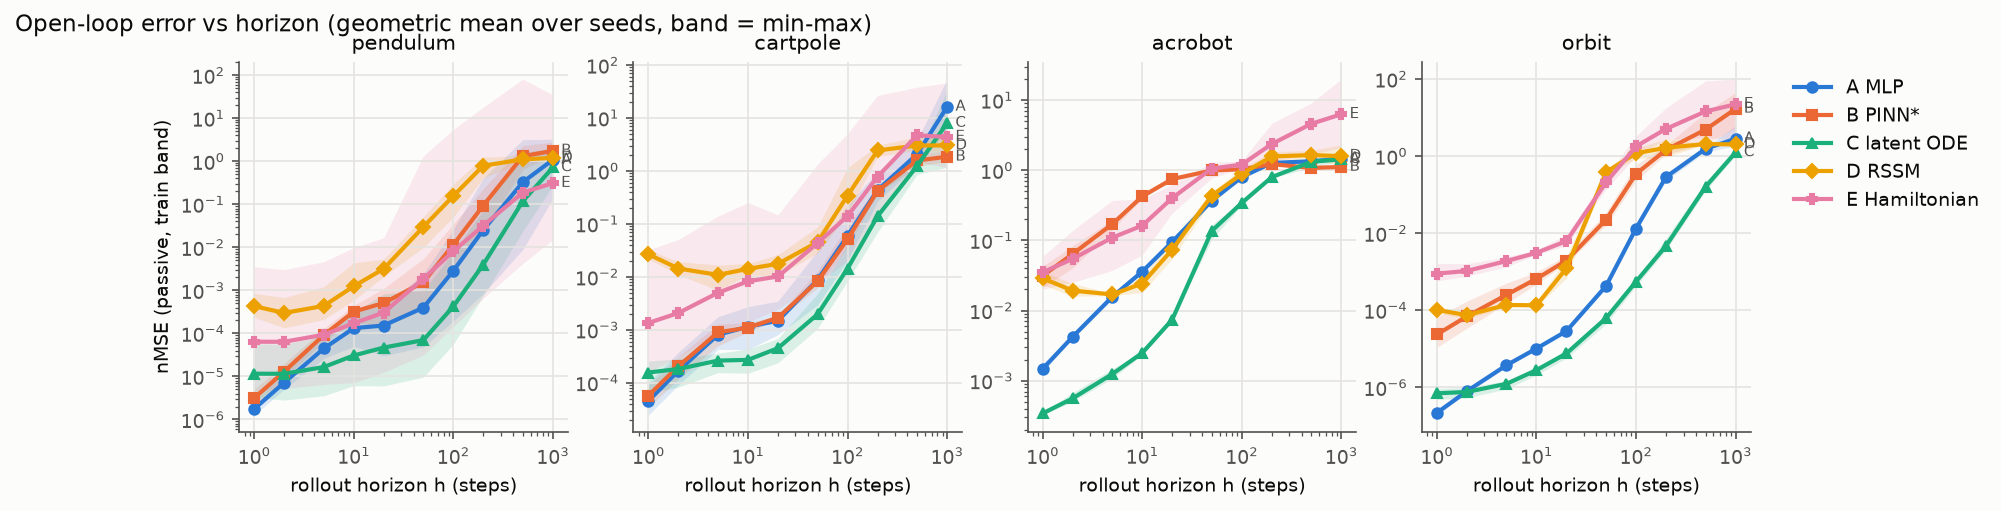
\includegraphics[width=0.49\linewidth]{error_vs_horizon.png}\hfill
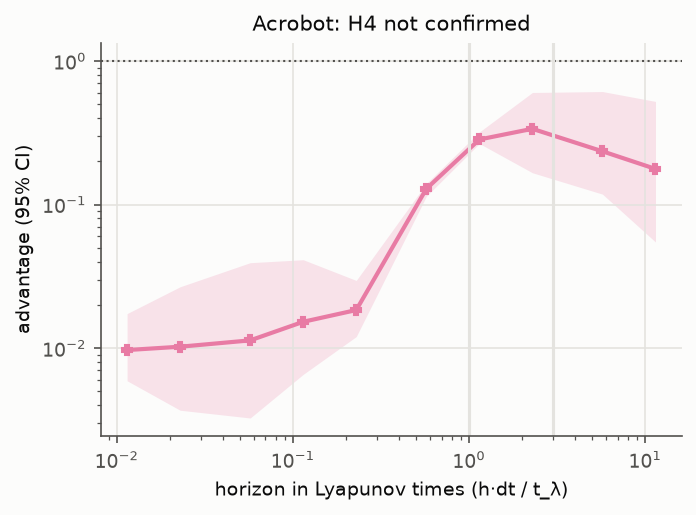
\includegraphics[width=0.49\linewidth]{advantage_vs_lyapunov.png}
\caption{Left: rollout nMSE against horizon for all models and systems. \E{} starts one to three orders
of magnitude above the baselines. Right: acrobot advantage of \E{} over the strongest baseline against
$h\,\Delta t/t_\lambda$; values below 1 mean \E{} is worse.}
\label{fig:curves}
\end{figure}

\paragraph{Replication.} On the two-body orbit, the energy-penalised latent ODE (C) drifts 0.21--0.37
against 256--393 for the plain MLP, and has lower 1000-step error (1.05--1.58 vs 1.8--6.1), reproducing,
with actions and three seeds, the qualitative result of an earlier informal study that motivated this
one (\url{https://github.com/Optimus2007/physics-informed-world-models}). On that system physics through the loss beats physics through the structure.

\section{Why it did not work}

\begin{enumerate}
\item \textbf{The guarantee is about the wrong energy.} Structure guarantees $H_\theta$ is conserved.
Any error in $H_\theta$ off the data manifold is then followed faithfully for $10^4$ steps. A soft
penalty on the true energy, as in C, corrects towards the right quantity; structure locks in the wrong
one. Conservation helps only when the learned energy is already right, which is the hard part.
\item \textbf{The bottleneck is too tight.} A $2n$-dimensional canonical latent leaves no room for the
encoder to represent anything the decoder needs beyond $(q,p)$, and the encoder must also discover a
canonical chart. Benchmarks of latent physical priors from pixels \citep{botev2021priors} reached a similar
conclusion; our state-vector results show the cost persists even without pixels.
\item \textbf{Seed variance dominates.} \E's failures are bimodal: a seed either finds a good $H_\theta$
or it does not. With three seeds and a worst-seed CI, one bad seed decides the verdict.
\end{enumerate}

\section{What we changed after freezing, and what it cost}

Amendment~1 (before any verdict): \E's training diverged to NaN on three systems. We added an L2 prior on
the latent (pinning the $p\to cp$ scale gauge of canonical coordinates), adaptive substeps where the
implicit-midpoint fixed-point iteration had not converged (a composition of symplectic steps is still
symplectic), dropped a latent-consistency term that diverged on the acrobot, and skipped non-finite
updates. \E{} thus received four diagnostic configurations on validation data and the baselines none,
an asymmetry that \emph{favours} \E{} and still did not rescue it. Amendment~2 is the H3 budget cut
above. Both are dated, recorded with reasons, and leave thresholds, metrics, splits and seeds unchanged.

\paragraph{Limitations.} Three seeds; one latent dimension ($2n$) for \E{} by design, which is a prior
the baselines do not get; no ensemble calibration analysis (the only ensembles are the pixel MBRL runs);
the H3 verdict rests on a floor effect and says nothing about the original protocol. A properly budgeted,
separately pre-registered pendulum-only H3 run is the obvious follow-up.

\paragraph{Reproducibility.} Code, configurations, the pre-registration, all run outputs and the verdict
script are public at \url{https://github.com/Shushant17711/hamiltonian-world-models} (MIT license);
\texttt{uv run pytest} checks that the frozen constants match the pre-registration hash.

\bibliographystyle{plainnat}
\bibliography{refs}

\end{document}
